% LaTeX coursework template with basic instructions and macros
%
% Edited: 2016-10-03 (Marc Deisenroth)
%
% you can compile with
%    pdflatex coursework.tex
%


\documentclass[11pt,twoside]{article}

\newcommand{\reporttitle}{Eigenvalues}
\newcommand{\reportauthor}{Matthew Pull}
\newcommand{\reporttype}{Mathematical Methods Coursework}
\newcommand{\cid}{01201299}

% include files that load packages and define macros
%%%%%%%%%%%%%%%%%%%%%%%%%%%%%%%%%%%%%%%%%
% University Assignment Title Page 
% LaTeX Template
% Version 1.0 (27/12/12)
%
% This template has been downloaded from:
% http://www.LaTeXTemplates.com
%
% Original author:
% WikiBooks (http://en.wikibooks.org/wiki/LaTeX/Title_Creation)
%
% License:
% CC BY-NC-SA 3.0 (http://creativecommons.org/licenses/by-nc-sa/3.0/)
% 
% Instructions for using this template:
% This title page is capable of being compiled as is. This is not useful for 
% including it in another document. To do this, you have two options: 
%
% 1) Copy/paste everything between \begin{document} and \end{document} 
% starting at \begin{titlepage} and paste this into another LaTeX file where you 
% want your title page.
% OR
% 2) Remove everything outside the \begin{titlepage} and \end{titlepage} and 
% move this file to the same directory as the LaTeX file you wish to add it to. 
% Then add \input{./title_page_1.tex} to your LaTeX file where you want your
% title page.
%
%----------------------------------------------------------------------------------------
%	PACKAGES AND OTHER DOCUMENT CONFIGURATIONS
%----------------------------------------------------------------------------------------
\usepackage{ifxetex}
\usepackage{textpos}
\usepackage{natbib}
\usepackage{kpfonts}
\usepackage[a4paper,hmargin=2.8cm,vmargin=2.0cm,includeheadfoot]{geometry}
\usepackage{ifxetex}
\usepackage{stackengine}
\usepackage{tabularx,longtable,multirow,subfigure,caption}%hangcaption
\usepackage{fncylab} %formatting of labels
\usepackage{fancyhdr}
\usepackage{color}
\usepackage[tight,ugly]{units}
\usepackage{url}
\usepackage{float}
\usepackage[english]{babel}
\usepackage{amsmath}
\usepackage{graphicx}
\usepackage[colorinlistoftodos]{todonotes}
\usepackage{dsfont}
\usepackage{epstopdf} % automatically replace .eps with .pdf in graphics
\usepackage{natbib}
\usepackage{backref}
\usepackage{array}
\usepackage{latexsym}

\usepackage{enumerate} % for numbering with [a)] format 



\ifxetex
\usepackage{fontspec}
\setmainfont[Scale=.8]{OpenDyslexic-Regular}
\else
\usepackage[pdftex,pagebackref,hypertexnames=false,colorlinks]{hyperref} % provide links in pdf
\hypersetup{pdftitle={},
  pdfsubject={}, 
  pdfauthor={\reportauthor},
  pdfkeywords={}, 
  pdfstartview=FitH,
  pdfpagemode={UseOutlines},% None, FullScreen, UseOutlines
  bookmarksnumbered=true, bookmarksopen=true, colorlinks,
    citecolor=black,%
    filecolor=black,%
    linkcolor=black,%
    urlcolor=black}
\usepackage[all]{hypcap}
\fi

\usepackage{tcolorbox}

% various theorems
\usepackage{ntheorem}
\theoremstyle{break}
\newtheorem{lemma}{Lemma}
\newtheorem{theorem}{Theorem}
\newtheorem{remark}{Remark}
\newtheorem{definition}{Definition}
\newtheorem{proof}{Proof}

% example-environment
\newenvironment{example}[1][]
{ 
\vspace{4mm}
\noindent\makebox[\linewidth]{\rule{\hsize}{1.5pt}}
\textbf{Example #1}\\
}
{ 
\noindent\newline\makebox[\linewidth]{\rule{\hsize}{1.0pt}}
}



%\renewcommand{\rmdefault}{pplx} % Palatino
% \renewcommand{\rmdefault}{put} % Utopia

\ifxetex
\else
\renewcommand*{\rmdefault}{bch} % Charter
\renewcommand*{\ttdefault}{cmtt} % Computer Modern Typewriter
%\renewcommand*{\rmdefault}{phv} % Helvetica
%\renewcommand*{\rmdefault}{iwona} % Avant Garde
\fi

\setlength{\parindent}{0em}  % indentation of paragraph

\setlength{\headheight}{14.5pt}
\pagestyle{fancy}
\fancyfoot[ER,OL]{\thepage}%Page no. in the left on
                                %odd pages and on right on even pages
\fancyfoot[OC,EC]{\sffamily }
\renewcommand{\headrulewidth}{0.1pt}
\renewcommand{\footrulewidth}{0.1pt}
\captionsetup{margin=10pt,font=small,labelfont=bf}


%--- chapter heading

\def\@makechapterhead#1{%
  \vspace*{10\p@}%
  {\parindent \z@ \raggedright %\sffamily
        %{\Large \MakeUppercase{\@chapapp} \space \thechapter}
        %\\
        %\hrulefill
        %\par\nobreak
        %\vskip 10\p@
    \interlinepenalty\@M
    \Huge \bfseries 
    \thechapter \space\space #1\par\nobreak
    \vskip 30\p@
  }}

%---chapter heading for \chapter*  
\def\@makeschapterhead#1{%
  \vspace*{10\p@}%
  {\parindent \z@ \raggedright
    \sffamily
    \interlinepenalty\@M
    \Huge \bfseries  
    #1\par\nobreak
    \vskip 30\p@
  }}
  



% %%%%%%%%%%%%% boxit
\def\Beginboxit
   {\par
    \vbox\bgroup
	   \hrule
	   \hbox\bgroup
		  \vrule \kern1.2pt %
		  \vbox\bgroup\kern1.2pt
   }

\def\Endboxit{%
			      \kern1.2pt
		       \egroup
		  \kern1.2pt\vrule
		\egroup
	   \hrule
	 \egroup
   }	

\newenvironment{boxit}{\Beginboxit}{\Endboxit}
\newenvironment{boxit*}{\Beginboxit\hbox to\hsize{}}{\Endboxit}



\allowdisplaybreaks

\makeatletter
\newcounter{elimination@steps}
\newcolumntype{R}[1]{>{\raggedleft\arraybackslash$}p{#1}<{$}}
\def\elimination@num@rights{}
\def\elimination@num@variables{}
\def\elimination@col@width{}
\newenvironment{elimination}[4][0]
{
    \setcounter{elimination@steps}{0}
    \def\elimination@num@rights{#1}
    \def\elimination@num@variables{#2}
    \def\elimination@col@width{#3}
    \renewcommand{\arraystretch}{#4}
    \start@align\@ne\st@rredtrue\m@ne
}
{
    \endalign
    \ignorespacesafterend
}
\newcommand{\eliminationstep}[2]
{
    \ifnum\value{elimination@steps}>0\leadsto\quad\fi
    \left[
        \ifnum\elimination@num@rights>0
            \begin{array}
            {@{}*{\elimination@num@variables}{R{\elimination@col@width}}
            |@{}*{\elimination@num@rights}{R{\elimination@col@width}}}
        \else
            \begin{array}
            {@{}*{\elimination@num@variables}{R{\elimination@col@width}}}
        \fi
            #1
        \end{array}
    \right]
    & 
    \begin{array}{l}
        #2
    \end{array}
    &%                                    moved second & here
    \addtocounter{elimination@steps}{1}
}
\makeatother


%%% Local Variables: 
%%% mode: latex
%%% TeX-master: "notes"
%%% End: 
 % various packages
% quick way of adding a figure
\newcommand{\fig}[3]{
 \begin{center}
 \scalebox{#3}{\includegraphics[#2]{#1}}
 \end{center}
}

%\newcommand*{\point}[1]{\vec{\mkern0mu#1}}
\newcommand{\ci}[0]{\perp\!\!\!\!\!\perp} % conditional independence
\newcommand{\point}[1]{{#1}} % points 
\renewcommand{\vec}[1]{{\boldsymbol{{#1}}}} % vector
\newcommand{\mat}[1]{{\boldsymbol{{#1}}}} % matrix
\newcommand{\R}[0]{\mathds{R}} % real numbers
\newcommand{\Z}[0]{\mathds{Z}} % integers
\newcommand{\N}[0]{\mathds{N}} % natural numbers
\newcommand{\nat}[0]{\mathds{N}} % natural numbers
\newcommand{\Q}[0]{\mathds{Q}} % rational numbers
\ifxetex
\newcommand{\C}[0]{\mathds{C}} % complex numbers
\else
\newcommand{\C}[0]{\mathds{C}} % complex numbers
\fi
\newcommand{\tr}[0]{\text{tr}} % trace
\renewcommand{\d}[0]{\mathrm{d}} % total derivative
\newcommand{\inv}{^{-1}} % inverse
\newcommand{\id}{\mathrm{id}} % identity mapping
\renewcommand{\dim}{\mathrm{dim}} % dimension
\newcommand{\rank}[0]{\mathrm{rk}} % rank
\newcommand{\determ}[1]{\mathrm{det}(#1)} % determinant
\newcommand{\scp}[2]{\langle #1 , #2 \rangle}
\newcommand{\kernel}[0]{\mathrm{ker}} % kernel/nullspace
\newcommand{\img}[0]{\mathrm{Im}} % image
\newcommand{\idx}[1]{{(#1)}}
\DeclareMathOperator*{\diag}{diag}
\newcommand{\E}{\mathds{E}} % expectation
\newcommand{\var}{\mathds{V}} % variance
\newcommand{\gauss}[2]{\mathcal{N}\big(#1,\,#2\big)} % gaussian distribution N(.,.)
\newcommand{\gaussx}[3]{\mathcal{N}\big(#1\,|\,#2,\,#3\big)} % gaussian distribution N(.|.,.)
\newcommand{\gaussBig}[2]{\mathcal{N}\left(#1,\,#2\right)} % see above, but with brackets that adjust to the height of the arguments
\newcommand{\gaussxBig}[3]{\mathcal{N}\left(#1\,|\,#2,\,#3\right)} % see above, but with brackets that adjust to the height of the arguments
\DeclareMathOperator{\cov}{Cov} % covariance (matrix) 
\ifxetex
\renewcommand{\T}[0]{^\top} % transpose
\else
\newcommand{\T}[0]{^\top}
\fi
% matrix determinant
\newcommand{\matdet}[1]{
\left|
\begin{matrix}
#1
\end{matrix}
\right|
}



%%% various color definitions
\definecolor{darkgreen}{rgb}{0,0.6,0}

\newcommand{\blue}[1]{{\color{blue}#1}}
\newcommand{\red}[1]{{\color{red}#1}}
\newcommand{\green}[1]{{\color{darkgreen}#1}}
\newcommand{\orange}[1]{{\color{orange}#1}}
\newcommand{\magenta}[1]{{\color{magenta}#1}}
\newcommand{\cyan}[1]{{\color{cyan}#1}}


% redefine emph
\renewcommand{\emph}[1]{\blue{\bf{#1}}}

% place a colored box around a character
\gdef\colchar#1#2{%
  \tikz[baseline]{%
  \node[anchor=base,inner sep=2pt,outer sep=0pt,fill = #2!20] {#1};
    }%
}%





%% Fast macro for column vectors
\makeatletter  
\def\colvec#1{\expandafter\colvec@i#1,,,,,,,,,\@nil}
\def\colvec@i#1,#2,#3,#4,#5,#6,#7,#8,#9\@nil{% 
  \ifx$#2$ \begin{bmatrix}#1\end{bmatrix} \else
    \ifx$#3$ \begin{bmatrix}#1\\#2\end{bmatrix} \else
      \ifx$#4$ \begin{bmatrix}#1\\#2\\#3\end{bmatrix}\else
        \ifx$#5$ \begin{bmatrix}#1\\#2\\#3\\#4\end{bmatrix}\else
          \ifx$#6$ \begin{bmatrix}#1\\#2\\#3\\#4\\#5\end{bmatrix}\else
            \ifx$#7$ \begin{bmatrix}#1\\#2\\#3\\#4\\#5\\#6\end{bmatrix}\else
              \ifx$#8$ \begin{bmatrix}#1\\#2\\#3\\#4\\#5\\#6\\#7\end{bmatrix}\else
                 \PackageError{Column Vector}{The vector you tried to write is too big, use bmatrix instead}{Try using the bmatrix environment}
              \fi
            \fi
          \fi
        \fi
      \fi
    \fi
  \fi 
}  
\makeatother

\robustify{\colvec} % short-hand notation
\usepackage{blkarray}
\addtolength{\oddsidemargin}{-.15in}
\addtolength{\evensidemargin}{-.15in}
\addtolength{\textwidth}{.3in}
\addtolength{\topmargin}{-.15in}
\addtolength{\textheight}{.3in}
\usepackage{graphicx}
\graphicspath{ {./images/} }

%%%%%%%%%%%%%%%%%%%%%%%%%%%%

% front page
\setcounter{secnumdepth}{0}
\usepackage[T1]{fontenc}
\usepackage{titling}
\title{ARM11 Project - Final Report}
\date{15th June, 2018}
\author{Matthew Pull, Alvin Lee, Ho Long Fung, Christopher Huang}
\begin{document}
\maketitle

%%%%%%%%%%%%%%%%%%%%%%%%%%%% Main document


\section{Group Organisation}
Our approach to this project is to divide the group into two sub teams. One subteam (Matthew and Alvin) would work on Part I - Emulator. The other subteam (Ho Long and Christopher) would work on Part II - Assembler. This plan allowed us to program the Emulator and Assembler concurrently.
\\\\
Each subteam met and further planned the structure of their assigned part, as well as the overall structure of the project. This included defining potential functions and the data types needed. We created a shared Google Drive folder in which we created several useful documents. One such document outlined internal deadlines that we set as a group. For each of the four parts of the project, we made summary notes about what we would need to implement. From these documents, tasks were assigned and tracked. We also split the main Git repository into "emulate" and "assembler" branchs to help organise our development.
\\\\
Within the subteams, after independently formulating solutions to the tasks, we met frequently to debug our programs. This process involved running the given test suite and performing additional tests for edge cases. Having fresh eyes look at an implementation helped to spot several syntactical and logical errors. Explaining our sections of code to each other also helped to uncover flaws or potential optimisations.  
\\\\
The group is working very well. This is evident by the completion of the emulator which passes all test cases. Good progress has also been made on the assembler, with most of the necessary helper functions (such as for parsing strings and bitwise operations) completed and organized into separate source files. We are all active on our group messaging platform and available to ask each other for advice. This will be especially useful when we look at Parts III and IV, as we will all be working on the same programs. 


\section{Emulator Implementation}
The emulator contains the following C files as well as the associated header (.h) files:
\begin{itemize}
\item emulate.c - Contains the main function coordinates the emulation of the Raspberry Pi.
\end{itemize}

We also created an "emulator\textunderscore utils" folder with the following files (with corresponding headers):
\begin{itemize}
\item decode.c - Converts a raw instruction to an decoded instruction struct via bit masking.
\item helper.c - Contains commonly used functions: swap\textunderscore endian (swaps the endianness of a 32-bit integer), check\textunderscore cond (identifies if a given instruction should be executed, based on the CPSR register), apply\textunderscore shift (performs various shift operations) and fill\textunderscore pipeline (fills the fetch-decode-execute pipeline immediately instead of requiring three cycles).
\item execute\textunderscore dp.c - Executes a given data processing instruction.
\item execute\textunderscore branch.c - Performs branching of +/- 32 MiB.
\item execute\textunderscore sdt.c - Allows for single data transfers used to load/store data from memory.
\item execute\textunderscore mult.c - Contains the multiply and multiply-accumulate operations.
\end{itemize}

We also defined the following header files with global constants and structs:

\begin{itemize}
\item instructions.h - Defines the enumeration of the five supported instruction types: HALT, (Data) PROCESSING, MULTIPLY, (Single Data) TRANSFER and BRANCH. The struct representing a decoded instruction is also defined, which holds the values of the different instruction parts (e.g. Condition field, Destination register etc).    

\item emulator\textunderscore machine\textunderscore details.h - This defines the constants of the emulated Raspberry Pi e.g. MEMORY\textunderscore ADDRESSES. A struct has also been defined to store the state of the machine, which consists of the memory array, register array, current instructions stored in each of three stages of the pipeline.
\end{itemize}


\section{Assembler Implementation}
Part II of the project was developed by Ho Long Fung and Christopher Huang. The sections below describe the structure and implementation of the assembler.
\subsection{Assembler Structure}
The assembler program opens the input ARM source file and creates an empty binary output file as specified by the command-line arguments. Then, the two-pass assembly process is executed with the following functions:
\begin{itemize}
\item firstPass - stores the labels and their corresponding memory addresses into a symbol table.
\item secondPass - processes each instruction by determining its type (Data Processing, Multiply, Single Data Transfer, Branch or Special), encoding it with a corresponding function and writing the result to the output file.
\end{itemize}
The project root folder contains the files assemble.c and assemble.h, where the main function and the firstPass and secondPass functions are defined. The rest of the assembler code contains the hash table implementation, encoding functions and utility functions. These are stored in the "assembler\textunderscore utils" folder with the following source and corresponding header files:
\begin{itemize}
\item hash\textunderscore table - Implementation of the symbol table, providing constructor / destructor, key-value insertion and lookup functions.
\item encode\textunderscore branch, encode\textunderscore dp, encode\textunderscore mult, encode\textunderscore sdt, encode\textunderscore special - functions for encoding each instruction type.
\item binary\textunderscore utils - Functions for common bitwise operations
\item parse\textunderscore utils - Functions for parsing instruction operands
\item string\textunderscore utils - Functions for comparing, searching and tokenizing strings
\item binary\textunderscore utils\textunderscore test.c, hash\textunderscore table\textunderscore test.c, string\textunderscore utils\textunderscore test.c, parse\textunderscore utils\textunderscore test.c - test cases for the utility functions
\end{itemize}

\subsection{Assembler Implementation Process}
\subsubsection{Planning and Assigning Tasks}
We decided on performing two passes over the source code instead of one. It is simpler to implement and dividing the assembly process into two parts improves readability and avoids code-clutter in the main function. We thought these benefits would outweigh the cost of slower execution time, which is only by a constant factor.
\\\\
We agreed on implementing the symbol table as an array-based hash table with chaining collision-resolution. A disadvantage is that the bucket size must be determined beforehand, which may be memory-inefficient if it is set higher than necessary. However, such an implementation is suitable for our purposes because it has fast average lookup and insertion speeds and the underlying data structures - array and singly linked list - are relatively simple and less error-prone to implement.
\\\\
We decided to work on the hash table simultaneously: Christopher would write the public functions (constructor/destructor, key-value insertion, lookup) and Ho Long would implement the hash function and the internal linked-list operations.
\\\\
We collaborated on the firstPass method and the input file loop in the secondPass. Then we divided the work based on the encoding functions for each instruction type, each of which would take an operator and the operands as string parameters, use string\textunderscore utils and parse\textunderscore utils to process them and use binary\textunderscore utils to encode them in the desired format. (Some of the functions require more parameters, such as the branch-instruction encoder that requires the symbol table.) The second-pass function would then use a switch statement to determine the type of the instruction and pass it to the corresponding encode function. Christopher would work on some of the Data-Processing (AND, EOR, SUB, RSB, ADD and ORR), Branching, and Special instructions, and Ho Long would work on the rest of the data processing (MOV, TST, TEQ, and CMP), Multiply, and Single Data Transfer instructions, allowing us to tackle specific parts of the problem in parallel.
\subsubsection{Development, Testing and Debugging}
We used CollabEdit, an online real-time code editor, to implement the first pass and the hash table. For the second-pass, although we worked on separate tasks, we shared parts of our code in CollabEdit to discuss potential improvements or suggestions for new helper functions that we could both use. For the rest, we each wrote code using the CLion IDE because its features features, such as on-the-fly code analysis and integration with external tools, help boost our productivity. We used Git for version control as required and worked on the assembler branch, separate from the emulator. Changes were committed whenever we reached a particular milestone, such as finishing an encoding function or fixing a major bug.
\\\\
After completing each encoding function, we ran the assembler against the corresponding test cases. For each failed case, we identified the problem by either inspecting the code or stepping through the code using GDB. Afterwards, we checked for memory leaks using Valgrind and ensured each dynamic memory allocation had a corresponding free() call, since they may go undetected even if all the test cases were passed. We added many error-checking statements and error messages to make it easier to identify the potential causes of bugs. In addition, we wrote and ran tests for utility functions and checked the results by visual inspection.
\\\\
To finalize the assembler, we examined the code together, discussing places where we could remove unnecessary variables, add comments and rename variables to improve readability and consolidate repeated statements in if-else blocks, and refactored them. For each change, we reran the test cases to ensure that the actual logic of the code was not altered. We merged the assemble branch into master, although further refactoring was done afterwards.
\subsubsection{Main Difficulties}
The symbol table implementation and the first-pass of the assembler were relatively straight-
forward, so the main difficulties are in the second-pass. With the LSL encoding function we found it difficult to construct the arguments for the MOV instruction and ended up having to do it manually. Parsing Operand2 and encoding constants to ARM immediate values requires some care. Assembling the LDR instruction with an immediate-value parameter required more steps than the others due to the multiple operand formats and the need to write values to the end of the file. The string parsing functions were tricky to get correct  due to pointer manipulation and memory issues. There are also some general design and refactoring issues such as avoiding code repetition and improving readability.

\section{GPIO on a Raspberry Pi}
The GPIO program works as described in the specification\footnote{Video evidence: bit.ly/GPIO-G16}. It was assembled using our completed assembler, emulated on our emulator and finally run on the Raspberry Pi. This can be seen in figure 1 in the Appendix.

\section{Extension: NintenDoC Arcade Machine}
\subsection{Introduction}
In the 90?s, many classic retro games such as DOOM\footnote{http://doom.wikia.com/wiki/Development\textunderscore of\textunderscore Doom} and Quake\footnote{http://quake.wikia.com/wiki/History\textunderscore of\textunderscore} were written in C. In a homage to those times, we decided to create a DoC-themed version of the Super Mario Bros platformer game (Super MariOh Baby!) housed in a retro arcade machine (NintenDoC).
\\\\
Galaxy Game (1971) was the very first coin-operated video game built and installed at Stanford University?s student union\footnote{http://infolab.stanford.edu/pub/voy/museum/pictures/display/5-GG-machine.htm}. Similarly, our arcade machine could be installed into the student union or DoC common room, which would not only provide hours of entertainment, but also give tech-savvy students the opportunity to produce their own games for the cabinet. The completed cabinet (without game) can be seen in figure 2 in the Appendix.

\subsection{Introduction}
We used the SDL2 development library because it satisfies our project requirements in several ways. It works natively with C, which is necessary since our extension must be written in that language. It provides graphics functions that allow us to render and animate 2D sprites. Its input-handling functionality enables us to interface the joystick and buttons built in the arcade machine with the game code.\footnote{https://wiki.libsdl.org/Introduction}
\\\\
The extension files are contained in the game folder, separate from the emulator and assembler code in src. It contains source and header files and two subdirectories: 
\begin{itemize}
\item data - contains 2D arrays representing the tiles in each level
\item images - the graphical resources, such as the sprites for tiles and Mario.
\end{itemize}

The file main.c contains code for initializing data structures, loading graphics resources and the game loop. game.c and game.h define global constants, such as Mario?s dimensions and the screen size, and various structs:
\begin{itemize}
\item The Game structure is the main component of the game. It contains fields such as the window, the graphics renderer, initialization and quit functions and the game state.
\item Each game character - Mario and the enemies - have a basic Core Object, which contain fields such as their current position, hitbox and whether they are alive or not.
\end{itemize}

Collision Detection is needed for game mechanics such as implementing jumping and Mario killing or being damaged by enemies. The files collision.c and collision.h contain code for detecting collisions between tiles or game characters.
\\\\
The files projectile.c and projectile.h contain a Projectile struct and functions to set its speed and target, which will form a basis for the flying objects in the game, such as as fireballs and Bullet Bill.
\\\\
Items in the game include coins and power-ups, such as the fire-flower which allows Mario to shoot enemies with fireballs and the mushroom which transforms him to Big Mario. The code for these are found in the files item.h and item.c.
\\\\
The files block.c and block.h contain code for the square blocks within the game. Blocks are either ? blocks, which reward Mario with either coins or powerups when jumping from underneath, or destructible bricks.
\\\\
input.c and input.h contains functionality for handling input from the joystick and buttons.

\subsection{Quality Assurance and Testing}
While testing we added continuous command-line output for the x and y coordinates of Mario and rendered the outlines of the Mario sprite and hitbox to ensure the movement and collisions are accurate. This approach was also used for the implementation of other features, as the command-line output made finding problems easy - without having to use a dedicated debugging tool.

We also ensured there are no memory leaks by using either the standard-library free() function or those provided by SDL (e.g. SDL\textunderscore FreeSurface and SDL\textunderscore DestroyTexture)).

At the start of the extension, we made a proof of concept work using SDL on the Raspberry Pi. From then on, however, we have tested the project on our own development machines, as this eliminates the long lead time involved in uploading to the Pi each time we make a small change. This significantly speeds up development time.

Ultimately, once the game is completed, the best way to test our machine is to spend hours playing the game trying to break it.

\section{Project Evaluation}
\subsection{Group Reflection}
Our unconventional approach was to divide the group into two sub teams. One subteam (Matthew and Alvin) would work on Part I - Emulator. The other subteam (Ho Long and Christopher) would work on Part II - Assembler. This plan allowed us to program the Emulator and Assembler concurrently. We then came together to complete Part III and Part IV.
\\\\
Each subteam met and further planned the structure of their assigned part, as well as the
overall structure of the project. This included defining potential functions and the data types needed. We created a shared Google Drive folder in which we created several useful documents. One such document outlined internal deadlines that we set as a group. For each of the four parts of the project, we made summary notes about what we would need to implement. From these documents, tasks were assigned and tracked. We also split the main Git repository into "emulate", "assembler" and ?game? branches to help organise our development and facilitate a good workflow. We would certainly do this for the next project.
\\\\
Within the subteams, we met frequently to debug our programs. This process involved running the given test suite and performing additional tests for edge cases. Having fresh eyes look at an implementation helped to spot several syntactical and logical errors. Explaining our sections of code to each other also helped to uncover flaws or potential optimisations. This worked particularly well and would definitely something we would do in the future.
\\\\
We believe that the group has worked very well with a very strong work ethic. This is evident by the timely completion of all parts of the project. The communication and organisation of the group was effective. Updating the respective Google Doc files during meetings helped to ensure everyone was on the same page. The Facebook Messenger chat was also helpful in ensuring asked queries could be resolved before the next meeting.
\\\\
There are some complications that we would want to prevent in future projects. During the initial stages of producing the extension, we investigated a number of potential graphics/physics libraries that could be used for the game. Many of these engines were poorly documented and hence we wasted a lot of time trying to get these libraries to work. Next time we will just pick the most commonly used, and well documented, library. 
\\\\
Although we communicated effectively, sometimes we weren?t as transparent about issues as we could have been. This would cause a slight hindrance to the overall workflow. If the rest of the team isn?t aware of an issue, the issue can?t be helped. For the next project, we will endeavour to be more candid about problems.
\\\\
An additional issue was the indecision between the group on agreeing which arcade game to produce. For a period of time we were switching between basing our game on Street Fighter or Super Mario. In future projects we will decide the direction of our project with more conviction and confidence.

\subsection{Individual Reflection}
\subsubsection{Matthew Pull}
I am very happy with our group - we have worked well together and accomplished a great deal in such a small amount of time. For the first 3 parts we split up the work by dividing into 2 teams, and I think that this was a major factor in how quickly we completed those first few parts. While we can definitely operative effectively as one large group - as is evidenced by the success of our extension - the smaller groups enabled us to focus on different pieces. We have held regular team meetings and I am very happy with the amount and quality of work achieved by all of my team members.
\\\\
My main strength has been coordinating the programming side of the extension and ensuring that all team members know what they should be working on. Fortunately this has been helped by having such a good team! I have also contributed a lot of the code and endured several all-night work sessions to get features implemented. I already had a good deal of programming experience before joining Imperial, and I have been happy to help others where needed - although this has rarely been necessary.
\\\\
With multiple all-night sessions, my sleep schedule drifted significantly from my other team members, which is something that I would try to avoid in the future as it did sometimes cause a delay in responding to questions that other team members had. Similarly I would be more transparent about potential problems - I have a tendency to try and deal with them myself before telling others, a trait that is not conducive to good team communication.


\subsubsection{Alvin Lee}
I believe that the group has integrated together very well. Over the past few weeks we have all contributed equally. 
\\\\
One of my strengths is organisation, I have been trying to push for certain internal deadlines (much to the chagrin of some of the team) as well as keeping track of progress. I have made sure that the rest of the team are aware of certain deadlines - such as WebPA assessments. One of my other strengths is coming up with ideas (e.g. for the extension). Although at times these ideas can be too overly ambitious.
\\\\
I thought that my weakness would be the fact that I don?t know the intricacies of Git. However throughout the project my teammates were able to teach me how to properly use Git for the purposes of version control on a large group project. I feel as though I would now be able to help others with Git. Additionally, I sought guidance from the rest of the team to figure out what in particular I had to implement. Despite this, the Google Doc and effective team communication meant that this was not a large issue. 
\\\\
In a different group I would push to keep up the strong work ethic that this current group had. This definitely helped to ensure the timely finish of the first three parts so that we had maximal time to work on our ambitious extension. Just in case a future group was not as dependable as the current one, I would try harder to break down the larger tasks into subtasks and delegate these accordingly.

\subsubsection{Ho Long Fung}
Overall I found this project to be a very rewarding experience. Not only was I able to improve my programming techniques and problem-solving skills, but also learned how to tackle a set of complex and technical tasks as a team.
\\\\
For Part 2, I think Christopher and I were able to split up the tasks and work in parallel effectively to completing the assembler. Through the project, I discovered that my strength is familiarity with C and data structures, as we were able to use C features, such as standard library functions, file I/O and structs, and write the assembler code without worrying about the syntax and focusing on the program?s logic instead. We also implemented the symbol table ADT without too much difficulty.
\\\\
I initially thought communication was my main weakness, but was able to overcome it by discussing ideas with the group, offering suggestions and pointing out issues while working on Part 2 and the extension. On the negative side, timing was an issue. Although our team was able to complete everything on time, Part 1 was finished earlier than Part 2. Although Alvin and Matt were productive while waiting for us to complete our part by reading up on C game development and organizing the hardware, the time lag was still not desired. In the future, I should aim to work on a tighter schedule and coordinate better with others to finish tasks more quickly.
\\\\
For the extension, I was mainly involved with the coding, but was not able to contribute the hardware and graphics design because of my lack of knowledge about it. Although it is not required that all team members should know how to do everything, I will likely learn those skills later on since they would definitely help with future projects.

\subsubsection{Christopher Huang}
I felt like I was a hindrance to the group near the beginning of the project, as I was much less familiar with C than everyone else.  However, with the help of my group mates I steadily became more familiar with the language.  Since then I was able to complete my assigned tasks at a reasonable rate.  I also felt that I was able to communicate well with the rest of the team.  One of the things I would like to work on for future projects is being more comfortable in voicing my own ideas, as I was lacking in that aspect this time around.  I definitely learnt a lot throughout this project, both from a technical standpoint and also on how to work effectively in a group.  

\newpage
\section{Appendex}
\begin{figure}[h]
    \centering
    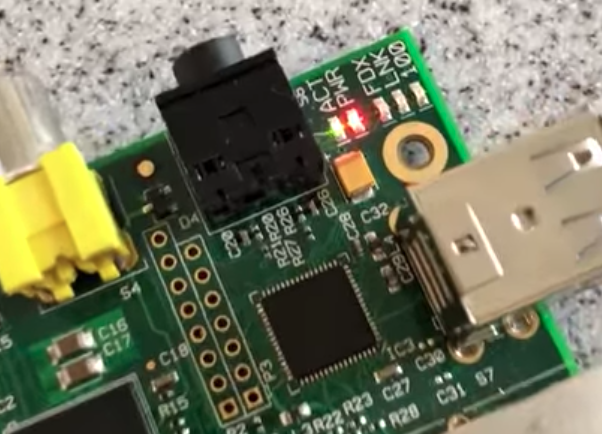
\includegraphics[width=\textwidth]{c_project_led}
    \caption{Blinking LED on the Raspberry Pi}
    \label{fig:led}
\end{figure}
\begin{figure}[h]
    \centering
    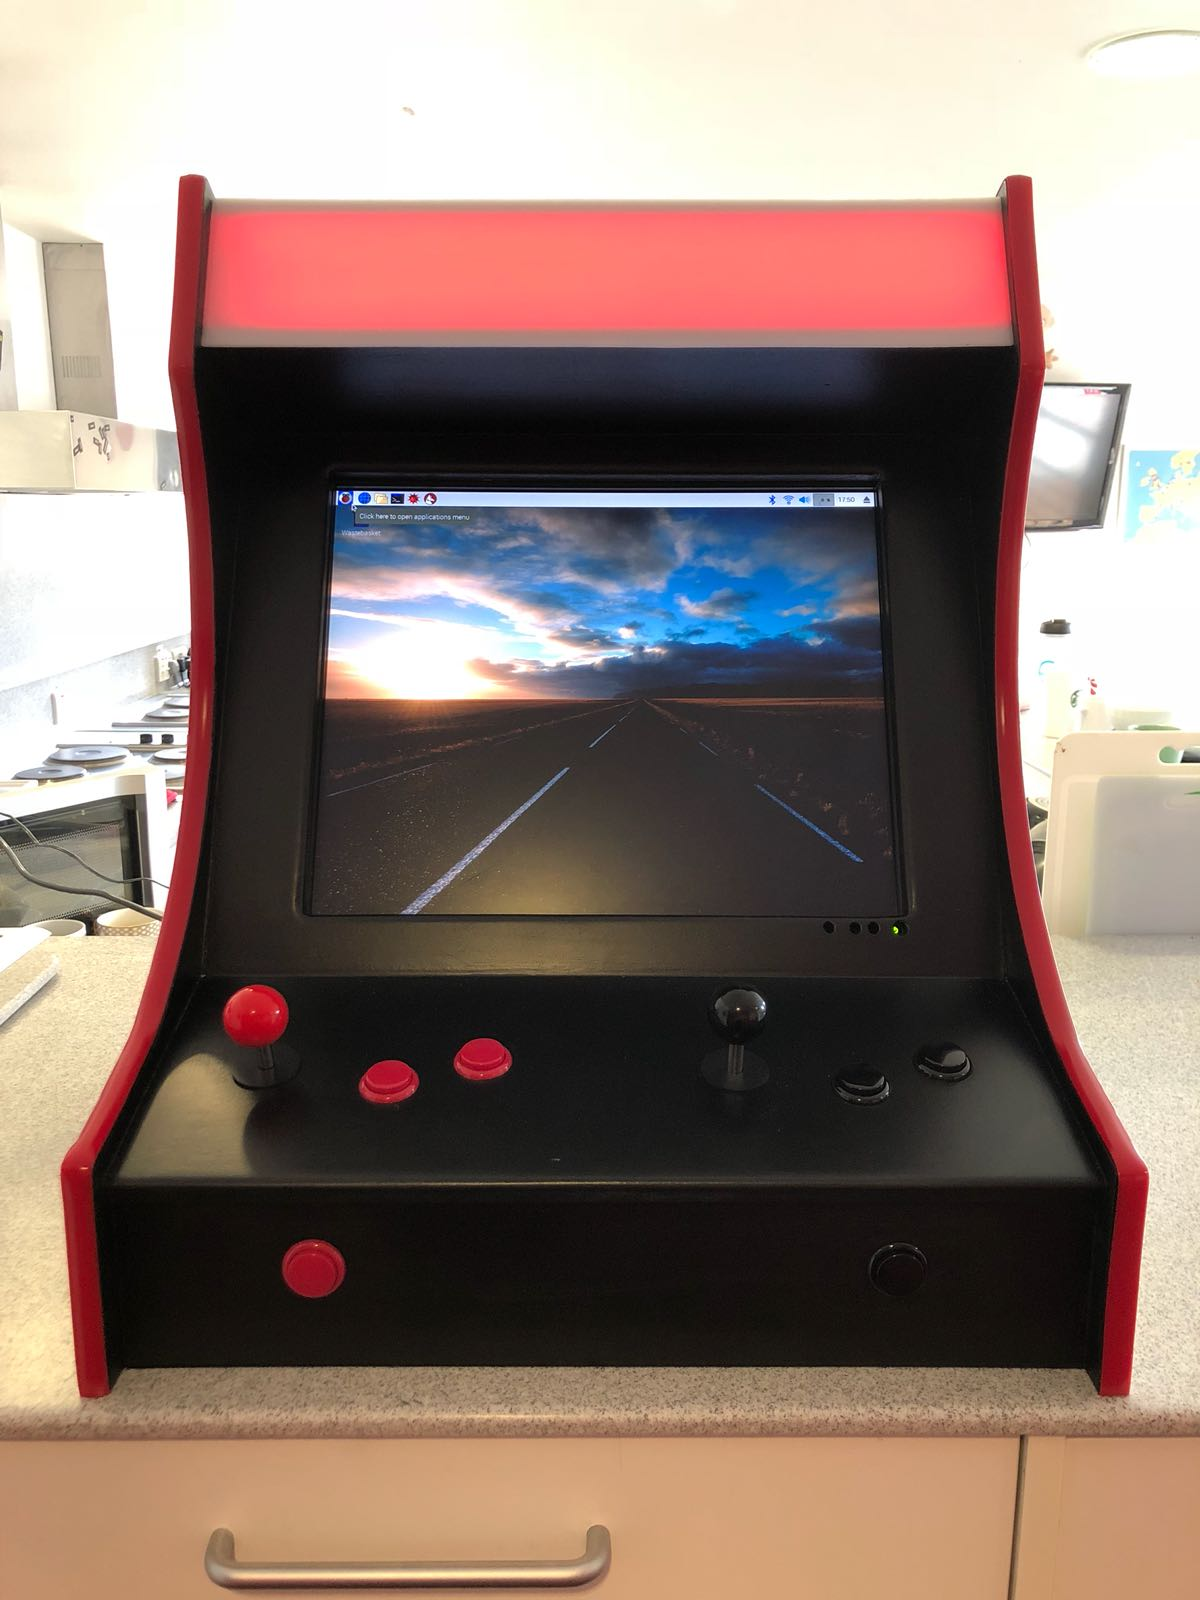
\includegraphics[width=\textwidth]{c_project_cabinet1}
    \caption{Arcade Cabinet}
    \label{fig:cabinet}
\end{figure}

\end{document}
%%% Local Variables: 
%%% mode: latex
%%% TeX-master: t
%%% End: 
